%%% Chapter 2 - Literature Reviews %%%
\chapter{Literature Reviews}

%%% Chapter Introduction %%%
This framework aims  to design and build an integrated system that consists of a centralised data management platform in conjunction with a network of interconnected sensors for the verification of sensors and the identification of anomalies will proceed more quickly as a result of this assembly.

%%% 2.1 Challenges It Faces Indicating The Need For This Research %%%
\section{Challenges It Faces Indicating The Need For This Research}
\lipsum[1]
\begin{figure}[!h]
	\centering
	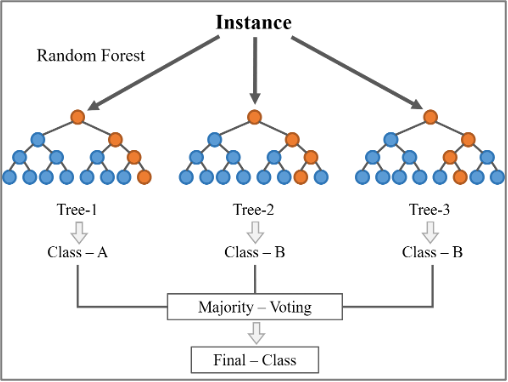
\includegraphics{chapter2/RandomForestClassification.png}
	\caption{Random Forest Classification}
	\label{fig:RandomForestClassification}
\end{figure}

From figure \ref{fig:RandomForestClassification} shows an optimized model that endeavors to heighten detection rates, precision, and processing times \cite{anderson2014engaging}. The innovative architecture integrates the Catboost classifier, melding Gradient Boosting (GB) with Decision Trees (DT). This synergy serves to curtail gradient estimation bias, consequently amplifying the model's generalization prowess. A significant attribute of this model is its utilization of GPU during the training phase, ensuring swifter computations.

	%%% 2.1.1 Fishbone Diagram %%%
	\subsection{Fishbone Diagram}
	\lipsum[1]
	\begin{figure}[!h]
		\centering
		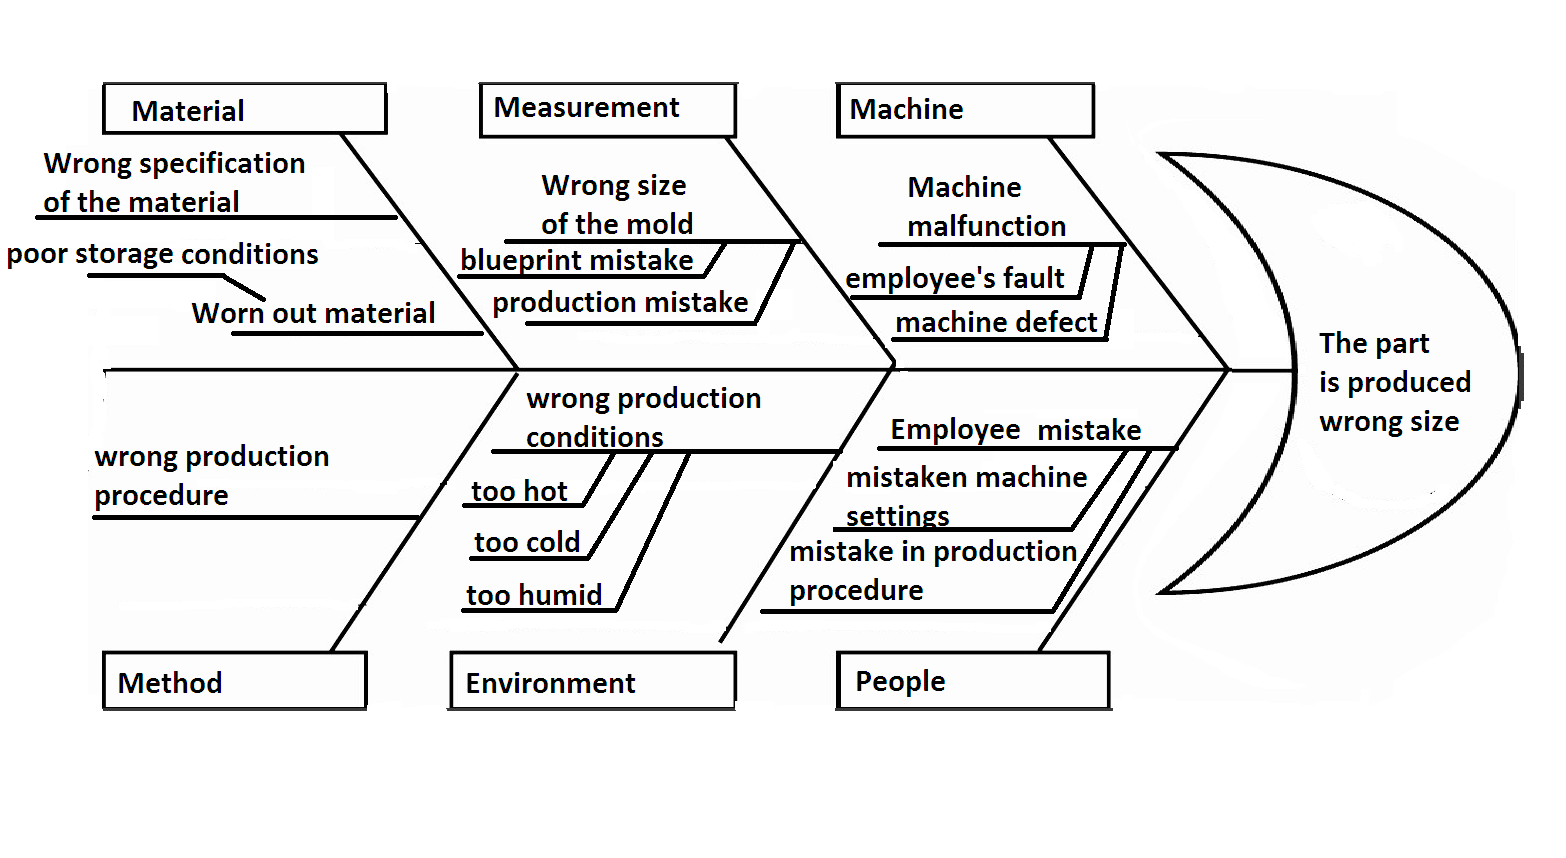
\includegraphics[height=7cm]{chapter2/fishbone.png}
		\caption{Fishbone Diagram}
		\label{fig:FishboneDiagram}
	\end{figure}
	
	From figure \ref{fig:FishboneDiagram} shows an optimized model that endeavors to heighten detection rates, precision, and processing times \cite{anderson2014engaging}. The innovative architecture integrates the Catboost classifier, melding Gradient Boosting (GB) with Decision Trees (DT). This synergy serves to curtail gradient estimation bias, consequently amplifying the model's generalization prowess. A significant attribute of this model is its utilization of GPU during the training phase, ensuring swifter computations.
	
	%%% Add more items depends on your research %%%
	
	%%% 2.1.X Conclusion %%%
	\subsection{Conclusion}
	\lipsum[1]
